\section{使用集成工具获取鼠标光标的位置}

控制器运行后,按下 \lstinline{Ctrl} \lstinline{Alt} \lstinline{Shift} \lstinline{5},将集成工具切换到模式 5。

将鼠标光标移动到欲确定坐标的位置,按下 \lstinline{Ctrl} \lstinline{Alt} 按键,罗技控制台中将输出鼠标光标的坐标位置。
注意,每次输出鼠标光标位置后间隔 0.5 秒才会允许输出下一个鼠标光标位置。为防止重复输出一样的结果,若本次获取到的的光标位置与上一次完全相同,则不再重复输出本次的光标位置。

\begin{figure}[H]
    \Centering
    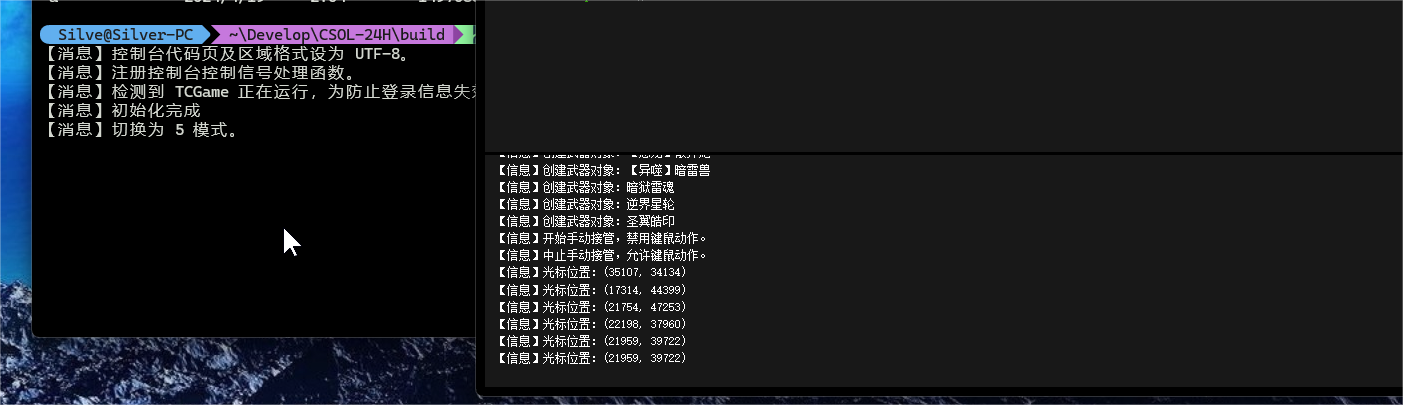
\includegraphics[width=\textwidth]{docs/assets/position.png}
    \caption{获取鼠标光标位置}
\end{figure}